%
% 計測自動制御学会システム・情報部門学術講演会2013原稿サンプルファイル
%                                           August 26, 2013
% 計測自動制御学会システム・情報部門学術講演会2011原稿サンプルファイル
%                                           April 28, 2011
% Based on 第7回計測自動制御学会制御部門大会原稿サンプルファイル
%                                           October 18, 2007
% Based on 第5回計測自動制御学会制御部門大会原稿サンプルファイル
%            近野敦 konno@space.mech.tohoku.ac.jp    March 05, 2005
%
% LaTeX2eとLaTeX209判別のための定義(以下3行)は科研費マクロkkhgrp.mac
% の定義を,作者の金沢大学青木先生の許可を得て利用させていただきました.
%
\newif\ifLaTeXe\LaTeXefalse
\expandafter\ifx\csname PackageError\endcsname\relax\LaTeXefalse
\else\LaTeXetrue\fi

\ifLaTeXe
  \documentclass{jarticle}
  \usepackage{SICE-SSI}
  \usepackage{otf}
  \usepackage{algorithm}
  \usepackage{algorithmic}
  \usepackage[dvips]{graphicx}
  \usepackage{subfigure}
  \usepackage{amsmath}
  \usepackage{longtable}
\else
  \documentstyle[SICE-SSI,epsbox]{jarticle}
\fi

\begin{document}
\title{複数解探索を考慮した分散型Bat Algorithm
% \thanks
% {本研究は○○で発表したものである.}
}
\author{○岩瀬拓哉\ \ \UTF{9AD9}野諒\ 上野史\  佐藤寛之\ \UTF{9AD9}玉圭樹 (電気通信大学)}

\abstract{
多峰性最適化問題における,従来の多点探索アルゴリズムは一つの最適解に収束する傾向にあるが,実問題への適用を考慮した時に複数の最適解及び局所解を探索する必要がある.多点探索アルゴリズムの中でも大域と局所の探索バランスに優れたBat Algortihmは探索する上で全個体の最良解を参照して移動するため,最終的に最適解に収束することから複数解を同時に探索することは困難である.本研究では各個体の探索領域を分割させるNiche Radiusを用いることで最適解だけでなく,局所解も同時に探索可能なBat Algorithmの構築をする.従来手法と提案手法の性能を比較するため,最適解と局所解の数が異なるパターンの多峰性関数を用いてシミュレーション実験を行った結果,全ての関数に対して従来手法は一つの最適解に収束していたが,提案手法では全最適解及び局所解を探索することができ,従来に対する変更点が有効であることを示した.


% 災害時における被災者の負傷具合を解空間内の局所解または最適解と見立てた時,負傷度合いに依らず多くの被災者を探索しなければならない.本研究では,様々な問題に適応して大域探索と局所探索の自動調整が可能であるBat Algorithmを用い,個体が同じ解に収束しないよう分散させるNiche Radiusによる複数解探索可能なアルゴリズムを構築する.
  }

\keyword{多点探索アルゴリズム,多峰性最適化問題,複数解探索, Bat Algorithm }

\maketitle\thispagestyle{empty}
\pagestyle{empty}

\section{はじめに}
近年,多点探索アルゴリズムは最適化問題において,一般的なメタヒューリスティック手法として用いられるようになった.多点探索アルゴリズムは特に非線形な問題に対しても適用することが可能であり,魚や鳥の群れをモデルにしたParticle Swarm Optimization(PSO)\cite{PSO}や,ホタルの光強度により互いのホタルが引き寄せられるFirefly Algorithm(FA)\cite{FA}は高次元な最適化問題に対して有効であることを示している.中でもBat Algorithm(BA)は大域探索と局所探索の性能を自動で切り替えるという点で優れたアルゴリズムである\cite{BA}.しかし多峰性最適化問題における,従来の多点探索アルゴリズムは全個体の中の最良解を参照して一点へ移動するため,探索終了時に一つの最適解に収束する傾向にあるが,実環境への適用を考慮した時に最適解だけでなく局所解を探索し,保持しておくことは非常に重要な意味を持つ.応用先の一例として,災害時における被災者を解,救助ロボットを個体と見立てた時に,不特定多数の被災者を探索することは人間にとって困難であり,複数の解を同時に探索しなければならない.\\ \
そこで本研究では,探索範囲の自動調整可能なBAを用い,各個体の探索領域を分割させることで個体の分散化を図る.探索空間のスケールと解の数から算出されるNiche Radius\cite{niche}を用いることで,予め各個体の探索領域を決定し,その探索領域内の最良個体から遠ざかる方向へ移動することで,個体同士が同じ解に留まらず,散らばるように改良する.従来手法の探索アルゴリズムに対して3つの変更をした.(i)大域探索: 分割探索領域内の最良解を参照;(ii)局所探索: 分割探索領域内の最良解付近に解候補を生成; (iii)ランダム探索: 選択した個体の分割領域内にランダムで解候補を生成.これらの変更により,従来手法と提案手法の探索性能を比較するため,発見した最適解及び局所解の数を評価尺度として,複数の異なる峰を持つ多峰性関数を用いてシミュレーション上で実験を行う.\\ \
本論文の構成はまず,2章で従来手法であるBAの概要とそのアルゴリズムについて説明し,3章にて提案手法の詳細と従来手法との変更点について述べる.4章では扱うベンチマーク関数とシミュレーション実験の内容及び,実験結果について記述し,5章で得られた結果に対して考察する.最後に6章にて,本論文の結論を述べる.

\section{Bat Algorithm}
\subsection{全体の概要}
Bat Algorithm(BA)は群知能アルゴリズムの一つで,対象物までの方向や距離を知るコウモリの特性(エコロケーション)を利用して周囲の状況を認知し,大域探索と局所探索が進むにつれて探索速度を徐々に落とし,探索性能を自動調節することが可能なアルゴリズムである.
% .BAにおいて,コウモリは自らの発する超音波の周波数を持ち,その周波数を調整するためのパラメータとしてラウドネス${A}$を用いる.
各個体の周波数${f_i}$,速度${v_i}$,位置${x_i}$は以下の式で定義し,更新される.
ラウドネス${A}$は,コウモリが対象物に近づくと値が減少し,移動距離も比例して短くなる.
コウモリの行動は以下3つで構成される.
\begin{itemize}
\item 大域探索: 各コウモリは位置${x_i}$において,自身が発する周波数${f_i}$の反響によって対象物との距離を測り,対象物に向かって速度${v_i}$で移動する.
\item 局所探索: 対象物近辺にコウモリを移動させる.
\item ランダム探索: 探索領域内にコウモリをランダムで移動させる.
\end{itemize}
\subsection{アルゴリズム}
BAで扱う各個体の周波数$f_i$,速度$v_i$,位置$x_i$は以下の式で定義される.
\begin{equation}
f_{i} =f_{min}+(f_{max}-f_{min}) \beta
\label{eq:freq} 
\end{equation}
% \begin{equation}
% d_i^{t-1}=x_*-x_i^{t-1}
% \label{eq:d}
% \end{equation}
\begin{equation}
v_i^{t+1}=v_i^{t}+(x_*-x_i^t)* f_i
\label{eq:vi}
\end{equation}
\begin{equation}
x_i^{t+1}=x_i^{t}+v_i^{t+1}
\label{eq:xi}
\end{equation}
個体番号を$i$とし,各個体の周波数${f_i}$は個体の速度を制限するパラメータであり,$[0, \ 1]$の区間で表される.ここでは${f_{min}=0}$,${f_{max}=1}$として設定し,$\beta$は0から1の乱数が割り当てられる.
局所探索では,全個体の最良解(グローバルベスト)$x_*$の周辺に新しい解候${x_{loc}}$を生成する.生成式は次の通りである.
\begin{equation}
\label{eq:loc}
x_{loc}=x_* + \epsilon A_i^t
\end{equation}
パラメータ$\epsilon$は1 $\times$ $D$次元の配列で$[-1, \ 1]$区間のランダムな値が割り当てられる. ランダム探索では解探索空間にランダムで新たに解候補を生成する.生成式は以下の通りである.
\begin{equation}
\label{eq:rnd}
x_{rnd}=x_{lb} + (x_{ub} - x_{lb})*rand(1,D)
\end{equation}
解探索空間の上限と下限をそれぞれ$x_{ub}$,$x_{lb}$とし,$rand$は0から1までの乱数が入る.
以上より各個体の解候補${x_i^{t+1}}$,${x_{loc}}$,あるいは$x_{rnd}$の評価値が各個体の最良解(パーソナルベスト)$x_{i*}$より良ければ更新され,同時にラウドネス$A$とその反射波であるパルスレート$r$も以下の式に基づいて更新される.
\begin{equation}
\label{eq:loud}
A_i^{t+1}= \alpha A_i^t
\end{equation}
\begin{equation}
\label{eq:pulse}
r_i^{t+1}=r_i^t[1-exp(- \gamma t)]
\end{equation}
解を更新する度にラウドネス$A_i$は徐々に減少し,それに比例して評価頻度を下げていく.対してパルスレート$r_i$は増加していき,探索が進むにつれて局所探索頻度が減少する.\\ \
従来のBAの疑似コードは以下のAlgorithm 1に記す.

\begin{algorithm}[H]
\caption{Bat Algorithm}
\label{code:ba}
\begin{algorithmic}[1]
\REQUIRE 評価関数 $F(x)$の設定
\STATE 各個体$x_i(i=1,2,...,N)$と速度$v_i$の初期化
% \STATE Niche Radiusの算出 [eqs.(\ref{eq:lambda}), (\ref{eq:NR})]
\STATE 周波数$f_i$の定義 [eq.(\ref{eq:freq})]
\STATE パルスレート$r_i$とラウドネス$A_i$の初期化
\WHILE{(t $<$ Max Iteration)}
\FOR{i=1 to N}
\STATE 大域探索: 新しい解候補$x_i^{t+1}$の生成と速度$v_i$の更新 [eqs.(\ref{eq:vi}),(\ref{eq:xi})]
% \ELSE
% \STATE Continue
% \ENDIF
\IF{($rand>r_i$)}
\STATE 局所探索: グローバルベスト$x_*$近辺に新しい解候補$x_{loc}$を生成 [eq.(\ref{eq:loc})]
\ENDIF
\STATE ランダム探索: 解空間に解候補の生成 [eq.(\ref{eq:rnd})]
\IF{($rand<A_i \ \& \ F(x_i),F(x_{loc}),F(x_{rnd})<F(x_{i*})$}
\STATE 新しい解の評価と更新
\STATE パルスレート$r_i$の増加とラウドネス$A_i$の減少 [eqs.(\ref{eq:loud}),(\ref{eq:pulse})]
\ENDIF
\ENDFOR
\STATE t=t+1
\ENDWHILE
\end{algorithmic}
\end{algorithm}

% \subsection{従来手法の問題点}
% BAの全ての探索において,最良解を参照しているために,最終的に最適解に収束してしまう問題がある.そこで本研究では,最良解の参照を避け,適切な探索範囲を与えることで問題の解決を図る.

\section{Niche Radius-based Bat Algorithm}
探索空間の分割方法の一つとしてNiche Radiusが挙げられる.Niche Radiusは探索空間のスケールと探索する解の数を元に個体の探索範囲を決定することのできる手法である.これにより,各個体が同じ解に留まることなく分散させ,従来のBAに以下3つの変更点を加えることで,最適解だけでなく局所解も同時に探索可能なNiche Radius-based Bat Algorithm(NRBA)を提案する.
\subsection{Niche Radiusの導入}
個体間同士の距離が近い場合に遠ざかる方向へ移動させる機構を持つNiche Radiusを用い,本研究では同じ解に個体が収束しないよう分散させ,Niche Radiusは解空間のスケールと最適解数から算出した距離(NR)であり,式(\ref{eq:lambda}),(\ref{eq:NR})で表される.

\begin{equation}
\label{eq:lambda}
\lambda =\frac{1}{2} \sqrt{(x_{ub}-x_{lb})^2}
\end{equation}
\begin{equation}
\label{eq:NR}
NR=\frac{\lambda}{\sqrt[D]{q}}
\end{equation}
$x_{ub}$,${x_{lb}}$は解空間の上限と下限を示し,${D}$は次元数,$q$は最適解の数を表す.本研究では探索する局所解と最適解の総数を$q$として扱う.
\subsection{変更点1:大域探索}
ここではNiche Radiusを使用し,従来手法の式(\ref{eq:vi}),(\ref{eq:xi})を次式のように変更を加えた.
\begin{equation}
\label{eq:nrvi}
v_i^{t+1}=v_i^t+(x_i^t-x_{NR*})*f_i
\end{equation}
\begin{equation}
\label{eq:nrxi}
x_i^{t+1}= \begin{cases}
x_i^t+v_i^{t+1} & (if \ d_i^t < NR) \\
x_i^t & (otherwise)
\end{cases}
\end{equation}
個体移動時のイメージ図をFig. \ref{fig:nr}に表す.各個体はNRを半径とした円の探索領域が決まっており,個体間距離${d_i}$がNRより小さい場合において,式(\ref{eq:nrvi})にてNR内の最良解${x_{NR*}}$を中心とした円から離れる方向へ個体${x_i^t}$が速度${v_i}$で移動する.またNR内に他の個体が存在しない,あるいは最良解$x_{NR*}$は移動をせず,その場所に留まる.この変更により,個体が同じ探索領域内に留まらず分散化をはかる.
\begin{figure}[h]
  \centering
  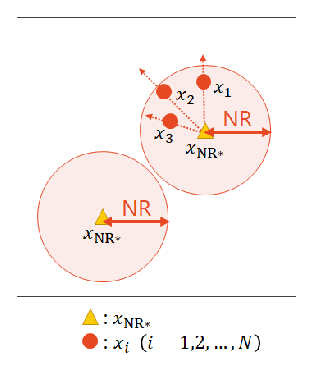
\includegraphics[width=0.5\linewidth]{eps/niche_radius.eps}
  \caption{Generating new solution candidates}
  \label{fig:nr}
\end{figure}

\subsection{変更点2: 局所探索}
次に局所探索性能を上げるため,各個体が持つNiche Radius内の最良解${x_{NR*}}$の周辺に新しい解候補${x_{loc}}$を生成するよう変更した.生成式は次の通りである.
\begin{equation}
\label{eq:nrloc}
x_{loc}=x_{NR*} + \epsilon A_i^t
\end{equation}

$\epsilon$は1 $\times$ $D$次元の配列で$[-NR, \ NR]$区間のランダムな値が割り当てられる.この変更により,個体を局所解へ収束するよう促す.
\subsection{変更点3: ランダム探索}
ランダム探索では各個体の持つNR内にランダムで解候補を以下の式のように生成する.
\begin{equation}
\label{eq:nrrnd}
x_{rnd}=x_i^t + rand(1,D,[-NR, NR])
\end{equation}
$[-NR, \ NR]$区間内の1×$D$次元の配列により現在位置$x_i^t$周辺に解候補を生成する.この変更では各個体を最適解あるいは局所解近辺へ移動させることで同じ場所に留まることを避ける. \\ \
% ラウドネス$A_i$は個体の評価値が更新する毎に徐々に値を減少させ,それとは対照的にパルスレート$r_i$は増加する機能を持つ.$\alpha$と$\gamma$は減衰係数を表し,シミュレーション上では$\alpha = \gamma = 0.9$として使用した.
提案手法のNRBAのアルゴリズムの疑似コードをAlgorithm 2に記す.

\begin{algorithm}[H]
\caption{Niche Radius-based Bat Algorithm}
\label{code:nrba}
\begin{algorithmic}[2]
\REQUIRE 評価関数 $F(x)$の設定
\STATE 各個体$x_i(i=1,2,...,N)$と速度$v_i$の初期化
\STATE 周波数$f_i$の定義 [eq.(\ref{eq:freq})]
\STATE パルスレート$r_i$とラウドネス$A_i$の初期化
\STATE Niche Radiusの算出 [eqs.(\ref{eq:lambda}), (\ref{eq:NR})]
\WHILE{(t $<$ Max Iteration)}
\FOR{i=1 to N}
\IF{($d_i<NR$)}
\STATE 大域探索: 新しい解候補$x_i^{t+1}$の生成と速度$v_i$の更新 [eqs.(\ref{eq:nrvi}),(\ref{eq:nrxi})]
% \ELSE
% \STATE Continue
\ENDIF
\IF{($rand>r_i$)}
\STATE 局所探索: 生成した解候補$x_i^{t+1}$近辺に新しい解$x_{loc}$を生成 [eq.(\ref{eq:nrloc})]
\ENDIF
\STATE ランダム探索: パーソナルベストの持つNR内に解候補の生成 [eq.(\ref{eq:nrrnd})]
\IF{($rand<A_i \ \& \ F(x_i), F(x_{loc}), F(x_{rnd})<F(x_{i*})$)}
\STATE 新しい解の評価と更新
\STATE パルスレート$r_i$の増加とラウドネス$A_i$の減少 [eqs.(\ref{eq:loud}),(\ref{eq:pulse})]
\ENDIF
\ENDFOR
\STATE t=t+1
\ENDWHILE
\end{algorithmic}
\end{algorithm}

% \subsection{図と表}

% \begin{figure}[t]
%   \centering
% \ifLaTeXe
%   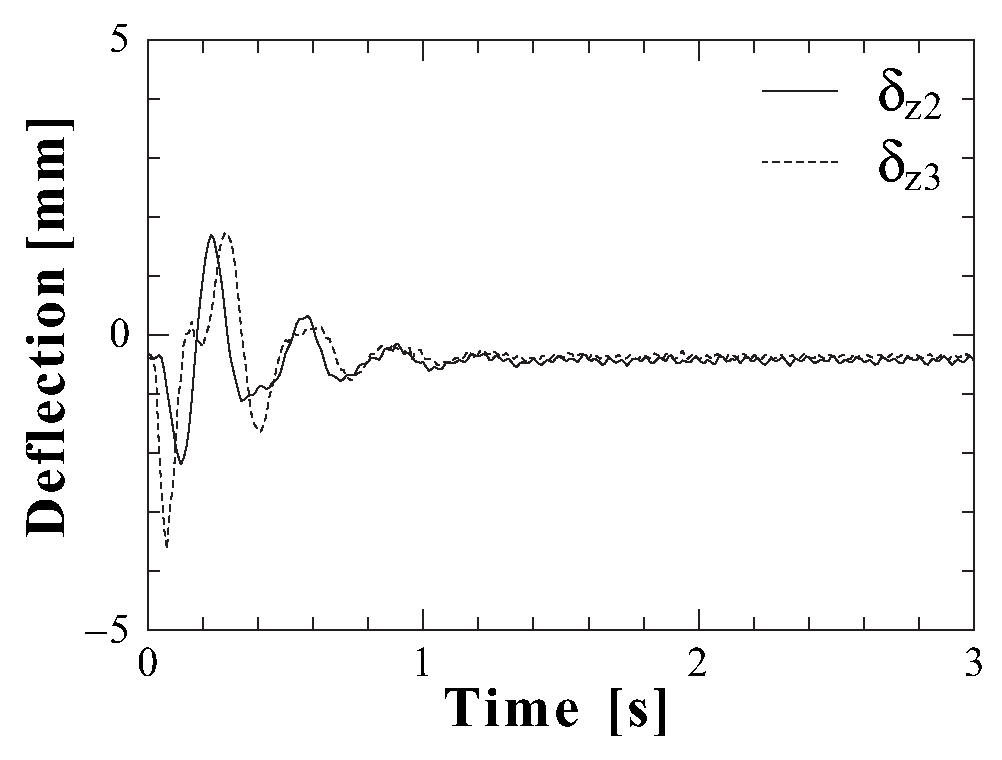
\includegraphics[width=0.5\linewidth]{fig1}
% \else
%   \psbox[width=0.55\linewidth]{fig1}
% \fi
%   \caption{A sample figure.}
%   \label{fig:samplefig}
% \end{figure}

% 図と表は,Fig. ~1,Table~1のように番号を振り
% (Fig. ~\ref{fig:samplefig}\ 参照),図説,図中の
% 説明文は英文で記入してください.本文で引用する場合も「Fig. ~1に示す」な
% どのようにFig. とTableを使用してください.

% 図や表中の文字は小さくなりすぎないよう気をつけてください.PDF原稿を作
% 成する際,図の画質が落ちないよう,注意してください.特にMicrosoft Word
% などで原稿を作成する際,JPEG画像を貼り付けると,一度圧縮されている画像
% が再圧縮されるので画像が劣化するようです.貼り付ける画像は,画質の良い
% (圧縮率の低い)画像を用いるか圧縮しない画像フォーマットを選ぶなど,各
% 自工夫し,最終的なPDFファイルにおいて画像が劣化しないよう注意してくだ
% さい.

\section{実験}
本研究では,最適解と局所解の数が異なる評価関数において,各手法の探索性能にどのような影響があるか調査する.次の4つのパターンの評価関数を用意し,従来手法と比較することで提案手法の探索性能を検証する..一つの最適解に対して複数の局所解を持つ;複数の最適解に対して同じ数の局所解を持つ;一つの最適解の数に対して一つの局所解を持つ;最適解のみ複数持つ.これらのパターンに適した多峰性関数を用いて実験を行う.
\subsection{問題設定}
実験で使用するベンチマーク関数の4つをFig. \ref{fig:all_func}に示す.Fig. \ref{fig:3d_griewank}からFig. \ref{fig:3d_himmelblau}は各評価関数の概形を表す.Fig. \ref{fig:cont_griewank}からFig. \ref{fig:cont_himmelblau}の各グラフの平面は2変数$x_1,x_2$空間を表しており,カラーバーは評価値を色濃度で表現したものとなる.本実験では最小化問題として,色濃度の濃い(評価値の低い)部分となる最適解と局所解の探索を目的とした.Table \ref{tab1}は各関数の探索領域と,最適解の評価値,最適解及び局所解の個数を示している.

\begin{table*}[t]
\caption{Measurement of Benchmark Functions}
\begin{center}
\begin{tabular}{c|c|c|c|c}
\hline
\textbf{Function} & ${F_1}$ & ${F_2}$ & ${F_3}$ & ${F_4}$  \\
\hline
\textbf{Search Domain} & $-10 \leq x_i \leq 10$ & $-2 \leq x_1 \leq 2,$ $-1 \leq x_2 \leq 1$ & $0 \leq x_i \leq 4$ & $-5 \leq x_i \leq 5$  \\
% & &  & & \\
\hline
\textbf{Fitness of global optimum} & 0 & -1.0316 & -1.8013 & 0  \\
\hline
\textbf{Num of global optima} & 1 & 2 & 1 & 4  \\
\hline
\textbf{Num of local optima} &  16 & 2 & 1 & 0  \\
\hline
% \multicolumn{4}{l}{$^{\mathrm{a}}$Sample of a Table footnote.}
\end{tabular}
\label{tab1}
\end{center}
\end{table*}

\begin{figure*}[h]
\begin{tabular}{cccc}
% \begin{center}

\renewcommand{\thefigure}{\alph{figure}}
\begin{minipage}{0.24\hsize}
\centering
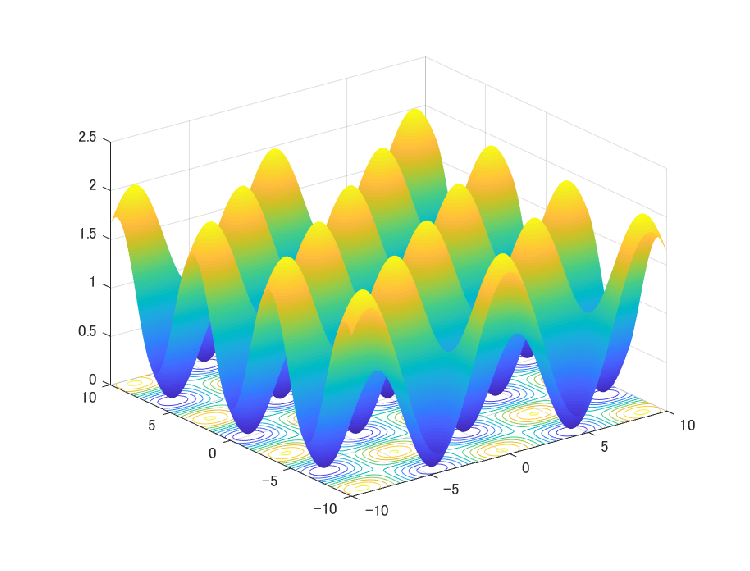
\includegraphics[width=1.0\linewidth]{eps/3d_griewank.eps}
\setcounter{figure}{0}
\caption{}
\label{fig:3d_griewank}
\end{minipage} 

\begin{minipage}{0.24\hsize}
\centering
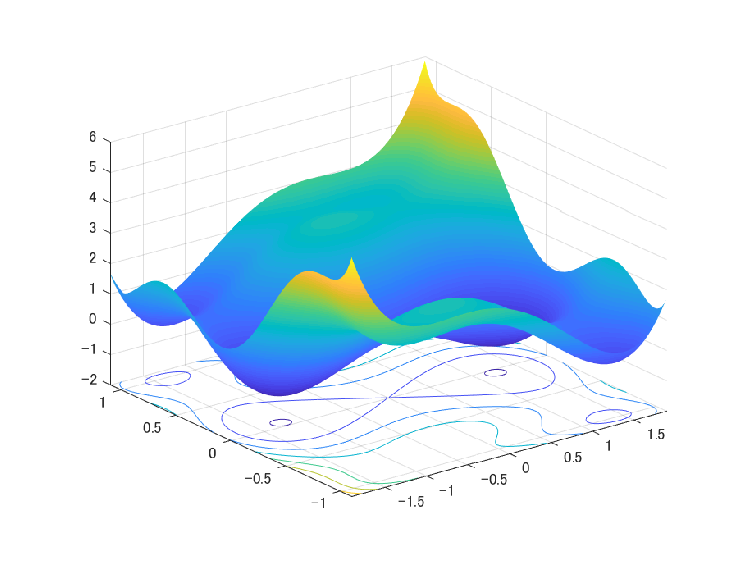
\includegraphics[width=1.0\linewidth]{eps/3d_sixhump_camel.eps}
\caption{}
\label{fig:3d_sixhump}
\end{minipage} 

\begin{minipage}{0.24\hsize}
\centering
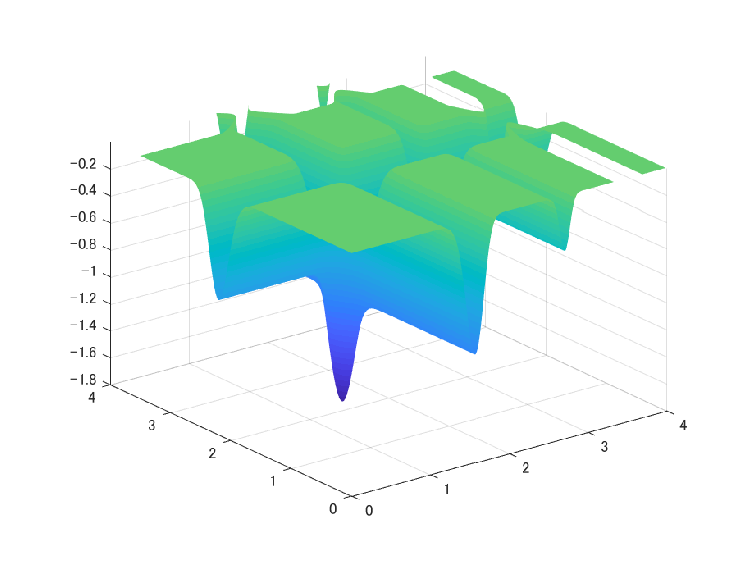
\includegraphics[width=1.0\linewidth]{eps/3d_michalewicz.eps}
\caption{}
\label{fig:3d_michalewicz}
\end{minipage} 

\begin{minipage}{0.24\hsize}
\centering
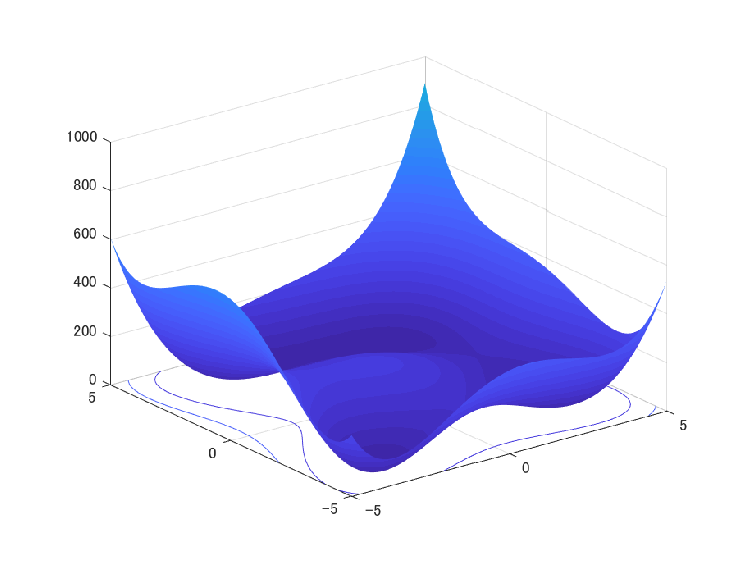
\includegraphics[width=1.0\linewidth]{eps/3d_himmelblau.eps}
\caption{}
\label{fig:3d_himmelblau}
\end{minipage}\\

\renewcommand{\thefigure}{\alph{figure}}
\begin{minipage}{0.24\hsize}
\centering
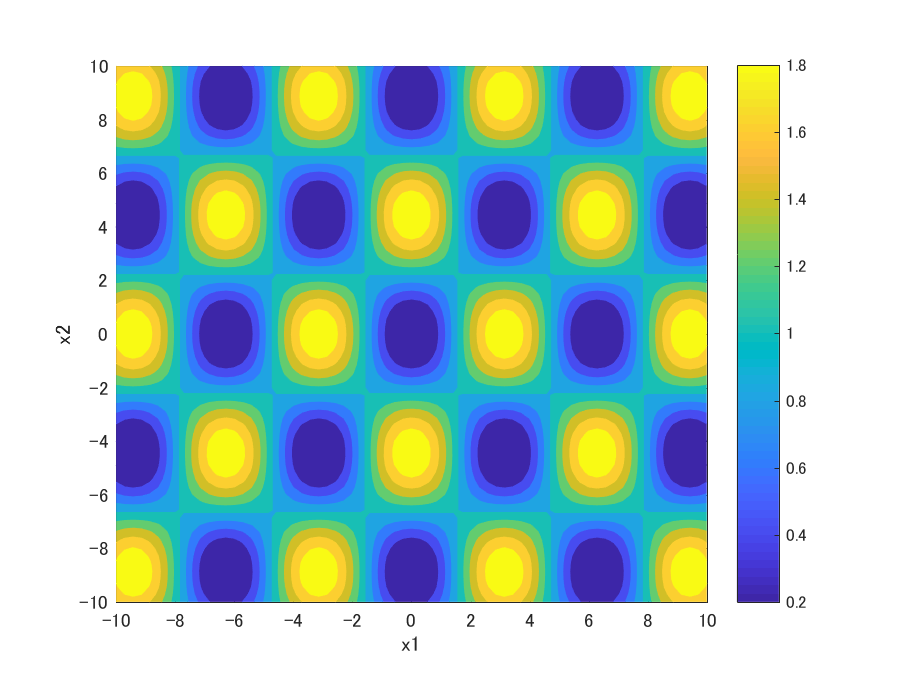
\includegraphics[width=1.0\linewidth]{eps/cont_griewank.eps}
\caption{}
\label{fig:cont_griewank}
\end{minipage} 

\begin{minipage}{0.24\hsize}
\centering
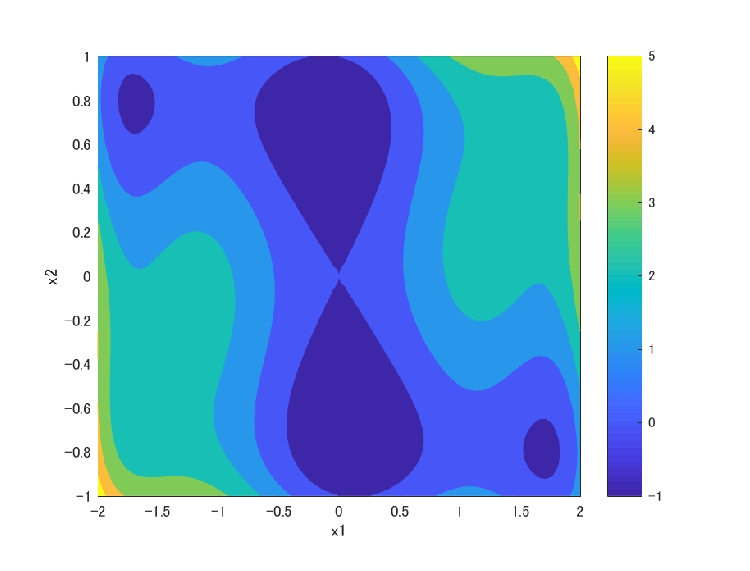
\includegraphics[width=1.0\linewidth]{eps/cont_sixhump_camel.eps}
\caption{}
\label{fig:cont_sixhump}
\end{minipage} 

\begin{minipage}{0.24\hsize}
\centering
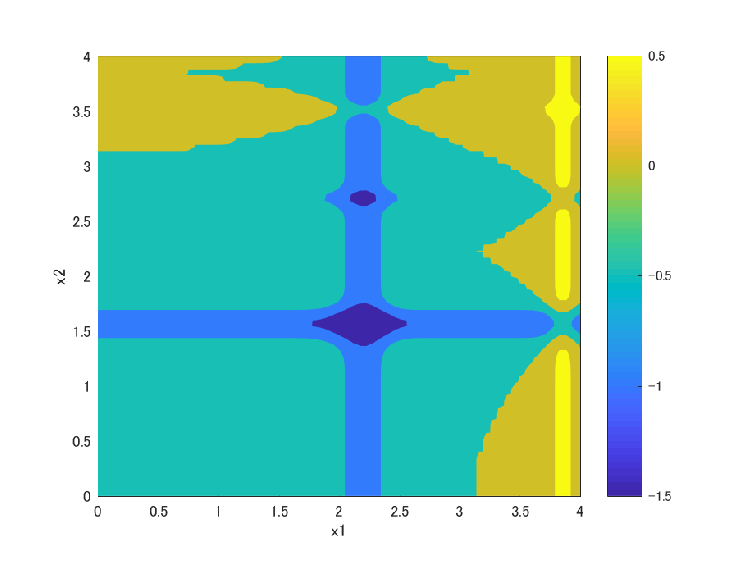
\includegraphics[width=1.0\linewidth]{eps/cont_michalewicz.eps}
\caption{}
\label{fig:cont_michalewicz}
\end{minipage} 

\begin{minipage}{0.24\hsize}
\centering
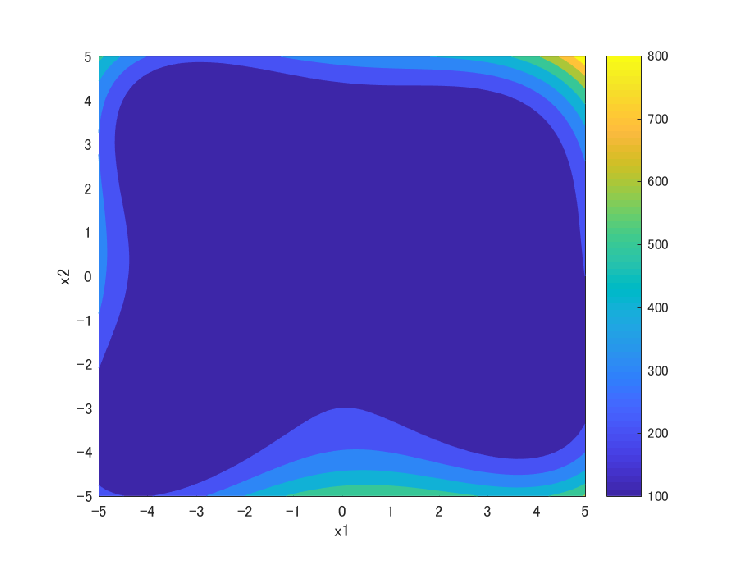
\includegraphics[width=1.0\linewidth]{eps/cont_himmelblau.eps}
\caption{}
\label{fig:cont_himmelblau}
\end{minipage} 

\end{tabular}
\setcounter{figure}{1}
\caption{Fitness landscape and contour of functions}
\label{fig:all_func}

\end{figure*}

\begin{description}
\item[Griewank Function]\mbox{}\\

多峰性関数の一つである,16個の局所解と1つの最適解を持つGriewank Function\cite{f1f3}を用いる(Fig. \ref{fig:3d_griewank}参照).評価関数の式は以下の通りである.
\begin{equation}
F_1(x_i)=\sum_{i=1}^D \frac{x_i^2}{4000}- \prod_{i=1}^D \cos( \frac{x_i}{\sqrt{i}})+1
\end{equation}
解空間の探索領域は$x_i \in [-10, \ 10]$である$(i=1,2)$.最適解の座標は$x_*=[0, \ 0]$で,その評価値は$F(x_*)=0$である.局所解の座標は$\pm x \approx [6.2800, \ 8.8769], [3.1400, \ 4.4385], [0, \ 8.8769],$ \\ $ [6.2800, \ 0], [9.4200, \ 4.4385]$となる.


\item[Six-Hump Camel Function]\mbox{}\\
% \subsubsection{$F_2$: Six-Hump Camel Function}
最適解と局所解が各2個存在するSix-Hump Camel Function\cite{f1f3}は以下の式で表される.
\begin{equation}
\label{eq:sixhump}
F_2(x_1,x_2)=(4-2.1x_1^2+ \frac{x_1^4}{3})x_1^2+x_1x_2+(-4+4x_2^2)x_2^2
\end{equation}
この関数における解空間の探索領域は$x_1 \in [-2, \ 2]$, \ $x_2 \in [-1, \ 1]$である.最適解の座標は$x_*=[0.0898, \ -0.7126], [-0.0898, \ 0.7126]$であり,その評価値は$F_3(x_*)=-1.0316$である.また局所解は$\pm x \approx [1.704, \ -0.7965]$に位置する.

\item[Michalewicz Function]\mbox{}\\
Michalewicz Function\cite{f1f3}の数式を以下に示す.
\begin{equation}
\label{eq:michalewicz}
F_3(x_i)=- \sum_{i=1}^D \sin(x_i)\sin^{2m}(\frac{ix_i^2}{\pi})
\end{equation}
最適解$x_*=[2.20, \ 1.57]$の評価値$F_3(x_*)=-1.8013$であり,局所解は$x \approx [2.203 \ 2.7115]$である.探索領域は$x_i \in [0, \ 4]$である($i=1,2$).

\item[Himmelblau Function]\mbox{}\\
Himmelblau Function\cite{f4}の関数式は次の通りとなる.
\begin{equation}
\label{eq:himmelblau}
F_4(x_1,x_2)=(x_1^2+x_2-11)^2+(x_1+x_2^2-7)^2
\end{equation}
評価関数に局所解は存在せず,最適解のみ4個持つ関数である.最適解の位置は各々$x_*=[3, \ 2]$,$[-2.805118, \ 3.283186]$,$[-3.779310,$ \\ \ $-3.283186],$ $[3.584458, \ -1.848126]$にあり,その評価値は$F_4(x_*)=0$である.探索領域は$x_i \in [-5, \ 5]$となる($i=1,2$).

\end{description}

\subsection{評価尺度}
本実験において,Congress on Evolutionary Computation(CEC2013)\cite{cec2013}のコンペティションで用いられた評価尺度であるPeak Ratio(PR)\cite{crowdingDE}により評価する.評価式は以下のように設定した.
\begin{equation}
\label{eq:PR}
PR=\frac{\sum_{run=1}^{MR}FPs}{TP*MR}
\end{equation}
Max Run(MR)は実験回数を表し,Found Peaks(FPs)は発見した解の数を,Total Peak(TP)は探索領域内の全最適解及び局所解数を表す.また最適解及び局所解の位置座標と最近傍個体とのユークリッド距離が0.1未満であれば,その解を発見したと定義する.

\subsection{パラメータの設定}
個体数$N=50$とし,各個体のパラメータ$A_i^0=1$, $r_i^0 \in [0,\ 1]$,$f_{max}=1, f_{min}=0$, $\alpha = \gamma = 0.9$と設定した.またTable \ref{tab1}より,探索領域の上限$x_{ub}$と下限$x_{lb}$,各評価関数の解の総数$q$として使用した.また次元数$D=2$,世代数を10000,実験回数$MR=30$とした.

\subsection{実験結果}
各評価関数について従来のBAと提案手法のNRBAにおける発見した解の数をTable \ref{tab2}に示す.表中のMean(平均値)とSD(標準偏差)は実験回数30回分での最終世代における発見した最適解及び局所解数の実験結果である.各手法の最終世代での個体の分布をFig. \ref{fig:results_ba}, \ref{fig:results_nrba}で表す.またグラフ中の赤い丸は個体の分布を示す.従来手法であるBAは全個体の最良解へ向かって進んでしまうため,全ての評価関数において,最適解あるいは評価値の高い局所解に収束した.しかしFig. \ref{fig:f4_ba}については局所解は存在しないが,最終世代では一つの最適解へ収束する結果となった.一方で提案したNRBAではFig. \ref{fig:results_nrba}から全評価関数において,全ての解に個体が到達しているように分布しているが,Table \ref{tab2}から実際に最適解や局所解の位置まで到達していないケースが多く見られた.また最適解や局所解に到達していない個体については用いた評価関数によって分布に偏りがあった.

\begin{figure}[pt]
\centering
\subfigure[$F_1$: Griewank]{
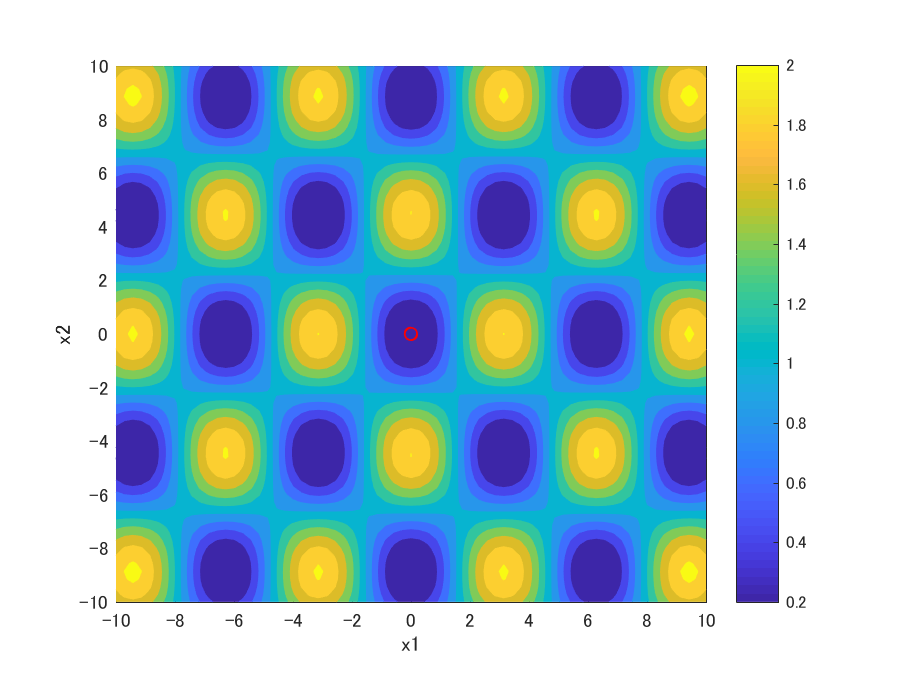
\includegraphics[width=0.9\linewidth]{eps/f1_ba.eps}
\label{fig:f1_ba}}
\subfigure[$F_2$: Six-Hump Camel]{
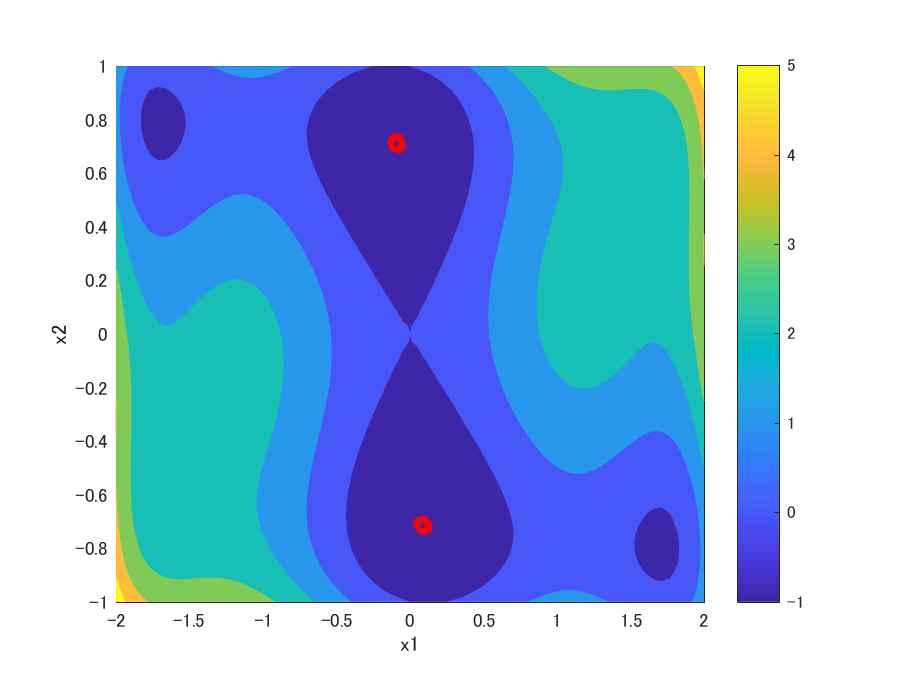
\includegraphics[width=0.9\linewidth]{eps/f2_ba.eps}
\label{fig:f2_ba}}
\subfigure[$F_3$: Michalewicz]{
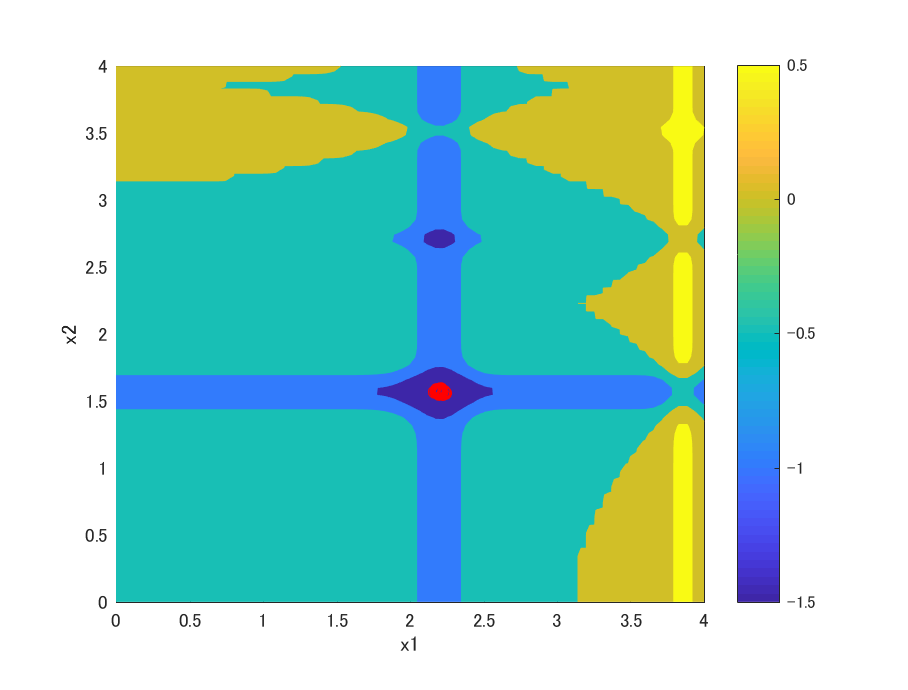
\includegraphics[width=0.9\linewidth]{eps/f3_ba.eps}
\label{fig:f3_ba}}
\subfigure[$F_4$: Himmelblau]{
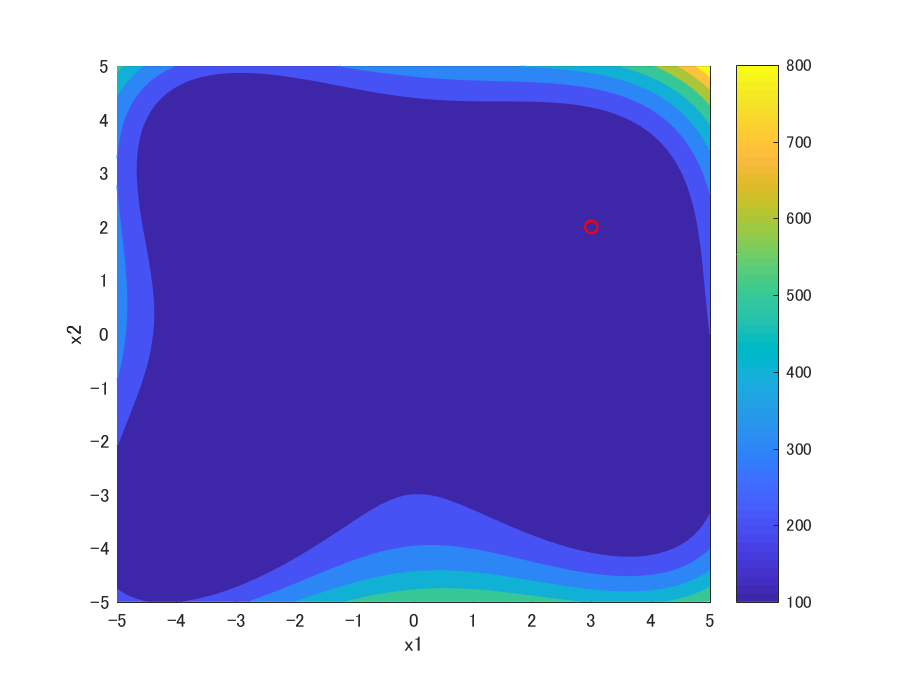
\includegraphics[width=0.9\linewidth]{eps/f4_ba.eps}
\label{fig:f4_ba}}

\caption{BA}
\label{fig:results_ba}
\end{figure}

\begin{figure}[pb]
\centering
\subfigure[$F_1$: Griewank]{
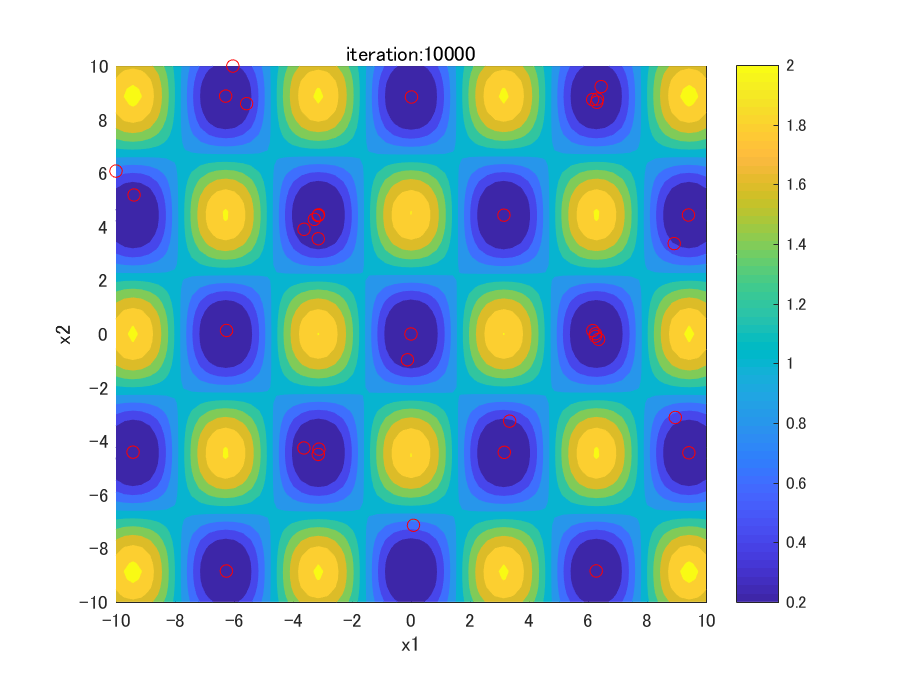
\includegraphics[width=0.9\linewidth]{eps/f1_nrba.eps}
\label{fig:f1_nrba}}
\subfigure[$F_2$: Six-Hump Camel]{
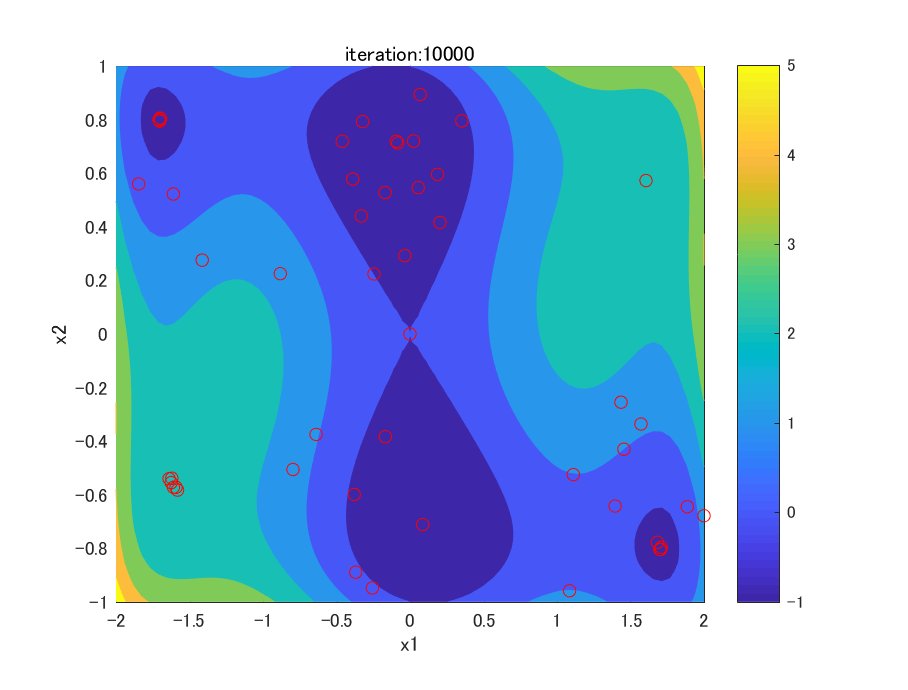
\includegraphics[width=0.9\linewidth]{eps/f2_nrba.eps}
\label{fig:f2_nrba}}
\subfigure[$F_3$: Michalewicz]{
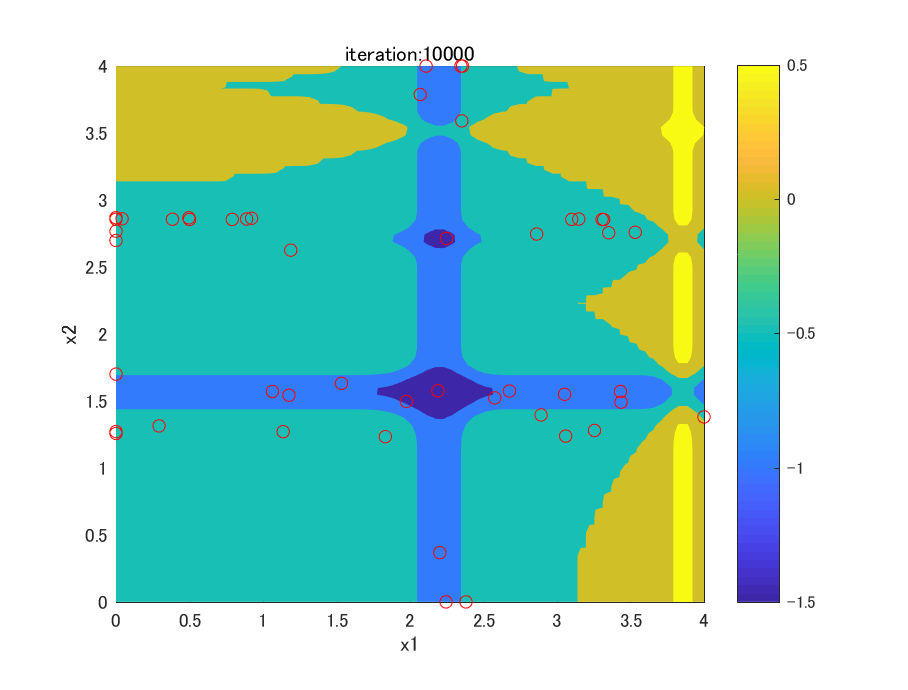
\includegraphics[width=0.9\linewidth]{eps/f3_nrba.eps}
\label{fig:f3_nrba}}
\subfigure[$F_4$: Himmelblau]{
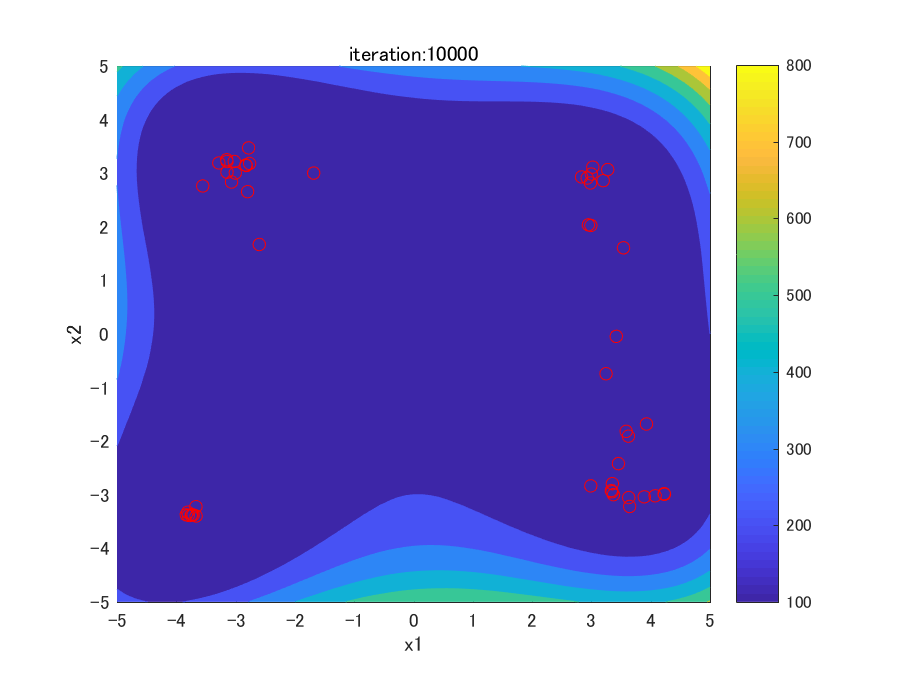
\includegraphics[width=0.9\linewidth]{eps/f4_nrba.eps}
\label{fig:f4_nrba}}

\caption{NRBA}
\label{fig:results_nrba}
\end{figure}

\begin{table*}[t]
\caption{Found Peaks and Peak Ratio}
\begin{center}
\begin{tabular}{c|c|c|c|c|c|c}
\hline
\multicolumn{1}{c|}{} & \multicolumn{3}{c|}{BA} & \multicolumn{3}{c}{NRBA}  \\
\hline
Function & Mean & SD & PR & Mean & SD & PR \\
\hline
$F_1$ & 1.0 & 0 & 5.88 \% & 11.767 & 1.667 & 69.22 \% \\
\hline
$F_2$ & 1.967 & 0.180 & 49.17 \% & 3.967 & 0.180 & 99.17 \% \\
\hline
$F_3$ & 1.0 & 0 & 50.00 \% & 1.4 & 0.490 & 70.00 \% \\
\hline
$F_4$ & 0.967 & 0.547 & 24.17 \% & 3.433 & 0.496 & 85.83 \% \\
\hline
% \multicolumn{4}{l}{$^{\mathrm{a}}$Sample of a Table footnote.}
\end{tabular}
\label{tab2}
\end{center}
\end{table*}
\section{考察}
全ての評価関数において,従来のBAより提案のNRBAのほうが探索した解の数および発見率が高かったことから最適解への収束を防ぎ,複数の局所解へ分散させることができた.また提案手法の探索性能の有効性を確かめるため,評価尺度による解の発見数及び発見率の結果と,最終世代の解の分布という観点から分析を行った.
\subsection{BA vs NRBA}
\subsubsection{解の発見数}
Table \ref{tab2}から従来手法のBAは全ての評価関数において一つの解へ収束する傾向が強かったが,$F_2$関数では2つの解を探索することができた.これは従来手法のアルゴリズムの解候補の生成において,全個体の最良解へ向かって探索をしていることが原因であると考えられる.提案手法のNRBAは全ての評価関数に対して,従来手法よりも発見した解の数が多く,最適解と複数の局所解を探索することができた.評価関数の中でも$F_2$関数,次いで$F_4$関数のPRの値が高いことから最適解のみ存在する場合と,最適解と局所解の評価値の差が小さい場合において提案手法の探索が有効に働いたと考えられる.また局所解を多く含む$F_1$関数や局所解の範囲が非常に狭い$F_3$関数では探索性能が落ちたことから今後の課題として手法を改良する必要がある.

\subsubsection{最終世代における解の分布}
Fig. \ref{fig:results_ba}から従来のBAは,最適解への収束が非常に強かった.しかし,Fig. \ref{fig:f2_ba}では2つの最適解に収束していたものの,Fig. \ref{fig:f4_ba}では複数の最適解へ収束することなく一つの最適解へ収束した.これは,$F_4$関数の方が探索領域が広く,評価値の数値の範囲も広いことから各個体の持つ評価値にバラつきが出やすく,一つの最適解へ収束したと考えられる.Fig. \ref{fig:results_nrba}より提案手法のNRBAは,Fig. \ref{fig:f1_nrba}では色濃度の濃い領域に各個体を分散させることができたが,Fig. \ref{fig:f2_nrba}, \ref{fig:f3_nrba}, \ref{fig:f4_nrba}では最適解や局所解でない場所に分布する個体も多く見られた.このことから従来手法から変更した,Niche Radius内の最良解より個体が遠ざかる機構が働いたと考えられる.以上より探索領域を分割し,各個体の探索領域内での大域探索性能を保ちながらも徐々に局所解へ収束させることが,解の発見率の増加に繋がったと考えられる.


\section{おわりに}
本論文では従来手法のBAについて,全個体の最良解を参照して一点へ集まってしまうという問題に対して最適解への収束を防ぎ,同時に複数の局所解を探索可能なNRBAを提案した.提案手法では従来手法から次の3点を変更した.(i)大域探索: 分割探索領域内の最良解を参照;(ii)局所探索: 分割探索領域内の最良解付近に解候補を生成; (iii)ランダム探索: 選択した個体の分割領域内にランダムで解候補を生成.提案手法の探索性能の検証するために従来手法と比較し,複数の最適解と局所解を持つベンチマーク関数を用いてシミュレーション上で実験した.結果,全てのベンチマーク関数において,従来手法より提案手法のほうが解の発見数及び発見率が高いことが分かった.このことから(i)の修正により全ての個体が最適解へ収束することを避け,(ii)より分割した探索領域内での探索性能を向上させ,(iii)より各最適解と局所解への収束を促すことにより,個体の分散化が有効に働いたといえる.\\ \
今後の課題としては全ての解を探索可能なアルゴリズムの性能向上と,複数解探索可能な他の最先端手法との性能比較,また実問題への適用を考慮した動的環境や個体数制限下においても探索性能を発揮できるアルゴリズムを構築する.


% \subsection{参考文献}

% 文献の引用は本文中に\cite{大会ホームページ}のように書き,本文の最後に
% まとめて記述します.次のフォーマットを推奨します.

% \noindent
% (a) 雑誌論文の場合

% \noindent
% 番号)  著者:論文題目,雑誌名,巻(太字)-号,始ページ/終ページ(年)

% \noindent
% (b) 単行本の場合

% \noindent
% 番号)  著者:書名,始ページ/終ページ,発行所(発行年)

% なお,本研究が他学会で発表済みの内容の場合,その文献を参考文献に挙げるとともに,脚注で明示して下さい.

\small
\begin{thebibliography}{10}
%%%%%%%%%%%%%%%%%%%%%%%%%%%%%%%%%%%%%%%%%%%%%%%%%%%%%%%%%%%%%%%%%%%%%%%%%%%%%%%

% \bibitem{大会ホームページ}
% {\tt http://www.sice.or.jp/org/SSI2015/}

% \bibitem{原稿執筆の手引き}
% 松野,中野:第7回計測自動制御学会制御部門大会サンプル原稿,
% 第7回計測自動制御学会制御部門大会予稿集,1/4(2007)
\bibitem{PSO}
Eberhart, R. C., and Kennedy, J. :“A New Optimizer Using Particle Swarm Theory”,
Proc. Sixth International Symposium on Micro Machine and Human Science (Nagoya, Japan), IEEE Service center, Pis-cataway, NJ, 39-43 (1995)

\bibitem{FA}
Yang, X. S. ”Firefly Algorithms for Multimodal Optimization”,in:Stochastic Algorithms: Foundations and Applications, SAGA 2009, Lecture Notes in Computer Sciences, Vol. 5792, pp. 169-178 (2009)

\bibitem{BA} Yang, X. S. “A Metaheuristic Bat-Inspired Algorithm”, {\it in: Nature Inspired Cooperative Strategies for Optimization (NISCO 2010) (Eds J.R. Gonzalez et al.)}, {\it Studies in Computational Intelligence}, Springer Berlin, 284, Springer, 65-74 (2010).

\bibitem{niche} D.Beasley, D.R. Bull, and R.R. Martin, "A sequantial niche technique for multimodal function optimization," {\it Evolutionary Computation}, vol. 1, no.2, pp. 101-125,1993.

\bibitem{f1f3}  Surjanovic, S. and Bingham, D. (2013). Virtual Library of Simulation Experiments: Test Functions and Datasets , Retrieved October 9, (2017)

\bibitem{f4} Himmelblau, D.(1972). Applied Nonlinear Programming. McGraw-Hill. ISBN 0-07-028921-2.

\bibitem{cec2013} X. Li, A. Engelbrecht, and M. G. Epitropakis, "Benchmark Functions for CEC'2013 Special Session and Competition on Niching Methods for Multimodal Function Optimization", {\it Evol. Comput.} Mach. Learn. Group, RMIT University, Melbourne, VIC, Australia, Tech. Rep., 2013.

\bibitem{crowdingDE} R. Thomsen,"Multimodal Optimization using Crowding-based Differential Evolution,"{\it In the IEEE Congress on Evolutionary Computation,}2004. CEC2004, vol.2, pp. 1382-1389, 19-23 June, 2004.

%%%%%%%%%%%%%%%%%%%%%%%%%%%%%%%%%%%%%%%%%%%%%%%%%%%%%%%%%%%%%%%%%%%%%%%%%%%%%%%
\end{thebibliography}
\normalsize

\end{document}
